\documentclass[a4paper,12pt,twoside]{article}
\usepackage[spanish]{babel}
\usepackage[utf8]{inputenc}
\usepackage{graphicx} %para insertar graficos/imagenes
\usepackage{amsmath} %para escribir matrices
\usepackage{amssymb}
\usepackage{upgreek}
\usepackage{amsfonts} %para poner \mathbb
\usepackage{float} %me deja usar la H de 'here' en los graficos para ponerlos donde yo quiera
\usepackage{anysize} %me permite definir los margenes como quiera
\usepackage{multirow} %para tablas con multicolumna
\usepackage{fancyhdr} % activamos el paquete
\usepackage{dcolumn}
\usepackage{multirow}
\usepackage{caption, subcaption}
\newcommand{\quotes}[1]{``#1''}
\captionsetup[table]{textfont=it,position=top}
\usepackage{booktabs}

\usepackage[output-decimal-marker={,}]{siunitx} %Para las unidades. Tengo la versión 2

\usepackage[font=footnotesize, labelfont=bf, margin=2.2cm]{caption}

\usepackage{fixme}
\fxsetup{
    status=draft,
    author=,
    layout=inline, % also try footnote or pdfnote
}

\usepackage[T1]{fontenc}

\newcommand{\grad}{$^\circ$}
\newcommand{\codigoMateria}{66.44}
\newcommand{\nombreMateria}{Instrumentos Electrónicos}
\newcommand{\nroTP}{1}
\newcommand{\descripcionTP}{Analizador de Espectro - Ruido}
\newcommand{\tituloTP}{Analizador de espectros - Ruido}
\newcommand{\facultad}{Facultad de Ingeniería}
\newcommand{\universidad}{Universidad de Buenos Aires}
\newcommand{\docentes}{Enrique Zothner}

\pagestyle{fancy} % seleccionamos un estilo
\fancyhead{}
\fancyfoot{}
\lhead{\nombreMateria \, (\codigoMateria)} % texto izquierda de la cabecera
\rhead{\facultad} % texto centro de la cabecera
\cfoot{\thepage}

\marginsize{2cm}{2cm}{1cm}{1.5cm} %izquierda, derecha, arriba, abajo

\newcommand{\Direcrotio}{./}
\newcommand{\HRule}{\rule{\linewidth}{1mm}}

\graphicspath{{./img/}}

\newenvironment{items}{
\begin{itemize}
  \renewcommand{\labelitemi}{$\bullet$}
  \setlength{\itemsep}{3pt}
  \setlength{\parskip}{1pt}
  \setlength{\parsep}{1pt}
}{
\end{itemize}}



\begin{document}

\begin{titlepage}

\thispagestyle{empty}

\begin{center}


\includegraphics[scale=0.15]{img/fiuba}\\[0.1cm]
\textsc{\universidad}\\[0.2cm]
\large{\textsc{\facultad}}\\[0.2cm]

\end{center}

\vfill

\begin{center}
\underline{\Large{\nombreMateria\, (\codigoMateria)}}
\end{center}

\vfill
\begin{center}

\end{center}
\vfill

\begin{center}
%\Huge{\textsc{ \tituloTP }}\\[.5cm]
	\begin{figure}[H]
		\centering
		%\includegraphics[width=.5\textwidth]{bessel}
	\end{figure}\HRule \\[0.1cm]
\Huge{\textbf{\descripcionTP}}\\[0.01cm]
\HRule\\[0.3cm]
\end{center}

\vfill



\begin{tabbing}
	FECHA: \today\\
\\
	INTEGRANTES:\hspace{-1cm}\=\+\hspace{1cm}\=\hspace{6cm}\=\\
		Carballeda, Ignacio	\>\>- \#91646\\
			\>\footnotesize{$<$carballeda.ignacio@gmail.com$>$}\\
\end{tabbing}

\begin{flushleft} \large
\emph{Docentes:}\\[.2cm]
\end{flushleft}
\begin{tabbing}
\docentes\\[.5cm]
\end{tabbing}

\vfill

\hrule
\vspace{0.2cm}

\noindent\small{\codigoMateria\, --- \nombreMateria \hfill \facultad}

\end{titlepage}


\newpage

\section{Ruido}
\subsection{Ruido estudiado como una señal}

Cuando querramos usar el analizador de espectros para medir ruido debemos tener en cuenta que por la naturaleza del mismo, este, indica un nivel que es mas bajo que el ruido que estamos midiendo. A continuacion vamos a ver porque sucede esto y como hacer para corregir este efecto.

Entendemos como ruido aleatorio una señal que tiene una amplitud instantanea distribuida de forma Gausiana (como en la figura \ref{ruido_gausiano}). Un ejemplo de esto es el ruido termico Johnson. Una señal asi no tiene componentes discretos en el espectro, por lo que no podemos tomar la amplitud de punto en particular para medir.
Debemos definir a que nos referimos cuando hablamos de \quotes{potencia de la señal}.

Si muestreamos una señal en un instante arbitrario de tiempo podriamos (en teoria) obtener su valor de amplitud. Pero necesitamos una medicion que exprese el nivel promedio de ruido a travez del tiempo. La potencia RMS satisface este requerimiento.

El filtro de video, y el promediador de video reducen las fluctuaciones pico a pico y nos pueden dar un valor estable. Debemos comparar este valor con la potencia o la tensión RMS. El valor RMS de una distribución Gausiana equivale a su desvio estandart $\upvarsigma$.

Vamos a comenzar como el analizador en modo display lineal. El ruido Gausiano es limitado en banda al pasar por la cadena de IF, y su envolvente adquiere una distribucion Rayleigh como en la figura \ref{ruido_ray}. El ruido que vemos en el display del analizador es la salida del detector de envolvente, es una envolvente distribuida como una Rayleigh de la señal de ruido de entrada. Para obtener un valor constante, un valor promedio, usamos el filtro de video o promediador. El valor medio de una distribucion Rayleigh es $1.253 \upvarsigma$. 

\begin{figure}[H]
    %\centering
    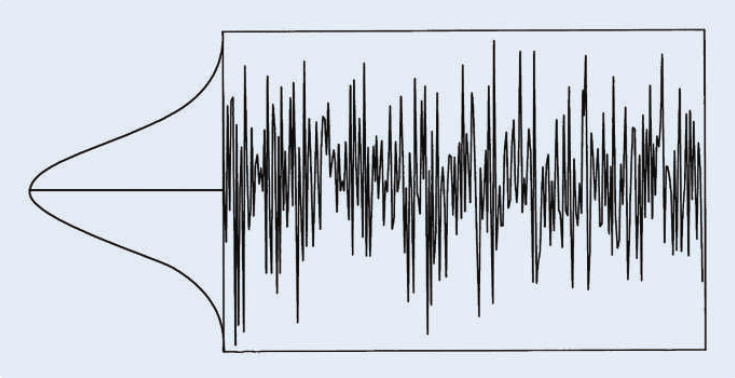
\includegraphics[width=0.8\textwidth]{../img/ruido_gausiano.png}
        \caption{El ruido aleatorio tiene una distribución Gausiana}
        \label{ruido_gausiano}
        \ref{ruido_gausiano}
\end{figure}

\begin{figure}[H]
    %\centering
    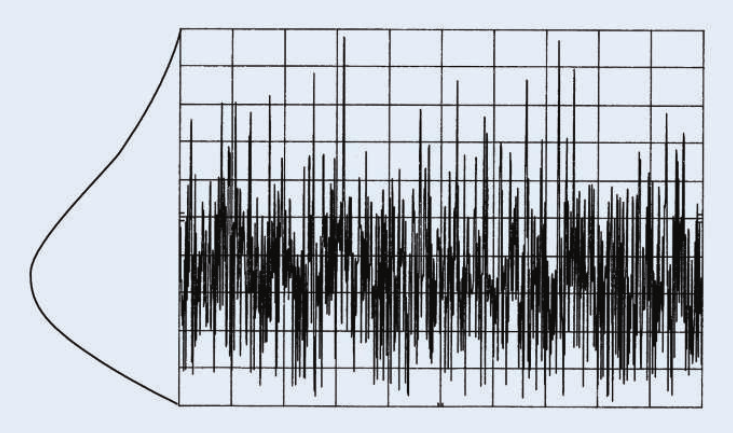
\includegraphics[width=0.7\textwidth]{../img/ruido_ray.png}
        \caption{La envolvente de una señal de ruido Gaussiano tiene una distribucion Rayleigh}
        \label{ruido_ray}
        \ref{ruido_ray}
\end{figure}

De todas formas nuestro analizador es un voltimetro calibrado que responde a picos para indicar el valor rms de una señal senoidal. Para convertir de calores pico a RMS, nuestro analizador escala su salida por $0.707$ (-3 dB). El valor promedio del ruido distribuido como Rayleigh es escalado entonces por el mismo factor, dandonos una lectura de $0.886 \upvarsigma$ ($1.05 dB$ por debajo de $\upvarsigma$). Para equiparar el valor medio mostrado por el analizador a tension RMS de la señal ruido de entrada debemos tener en cuenta el error introducido en el valor mostrado. Notar que este error no es ambiguo, este es un error constante que puede ser corregido agregando 1.05 dB al valor mostrado en el display.\newline

En la mayoria de los analizadores de espectro la escala del display controla la escala en la cual la distribucion de ruido es promedida tanto con el filtro de VBW o con la traza promediadora. Normalmente, usamos el display del analizador es modo logaritmico, y este modo se agrega al error en nuesta medicion de ruido.\newline

La ganancia de un amplificador logaritmico esta en funcion de la amplitud de la señal, los valores altos de ruido no son tan amplificados tanto como los valores pequeños. Como resutado, la salida del detector de envolventes es una distribucion Rayleigh sesgada, y el valor medio que obtenemos del filtro de video o promediado es otro que esta 1.45 dB mas abajo. En el modo logaritmico, entonces, la media o ruido promedio es mostrado 2.5 dB mas abajo.
Otra vez, este error no es ambiguo, y por lo tanto lo podemos corregir.\newline

Otro factor que afecta a las mediciones de ruido es el ancho de banda en el cual la medición es hecha. Un cambio en la resolución del ancho de banda (RBW) afecta el nivel mostrado del ruido interno generado por el analizador. Este RBW afecta en igual medida a las señales de ruido externas. Para comparar las mediciones hechas con diferentes analizadores, debemos conocer los anchos de banda usadod en cada caso.\newline

No solo los 2 o 6 dB del ancho de banda del analizador afectan la medida del nivel de ruido, la forma del filtro  de resolución tambien juega un papel importante.\newline

Para hacer posible las comparaciones, definimos un \quotes{ancho de banda de potencia del ruido}: el ancho de un filtro rectangular que permite pasar la misma potencia de ruido que el filtro del  analizador. Para un filtro cuasi-Gausiano en un analizador Agilent, el equivalente \quotes{ancho de banda de la potencia del rudo} es de 1.05 a 1.13 veces los 3 dB del ancho de banda, dependiendo de la selectividad del ancho de banda. Por ejemplo para un filtro RBW de 10KHz se tiene una \quotes{ancho de banda de potencia del ruido} en el rango de 10.5 a 11.3 KHz.\newline

Si usamos $10*\log(BW_{2}/BW_{1})$ para ajustar el nivel de ruido mostrado a lo que habriamos medido con \quotes{ancho de banda de potencia del ruido} del mismo valor que con nuestro ancho de banda de 3 dB, encontramos que los ajustes varian de: $10*log(10000/10500) = -0.21dB$ a $10*log(10000/11300)=-0.53 dB$. En otras palabras, si restamos algo entre 0.21 y 0.53 dB del nivel de ruido indicado, tendremos el \quotes{ancho de banda de potencia de ruido} que es conveniente para realizar los calculos. Para los siguientes ejemplos vamos a usar 0.5 dB como un compromiso razonable para la correccion del ancho de banda.
\newline

Vamos a considerar los factores de correccion para calcular el total de correcciones para cada modo de promediado:
\newline

\bold{Promediado Lineal}\newline
Distribución Reyleigh (modo lineal): $1.05$ dB \newline
3-dB/Ruido potencia ancho de banda:  $-0.50$ dB \newline
Correccion total: $0.55$ dB
\newline

\bold{Promediado Logaritmico}\newline
Distribución Reyleigh (modo logaritmico): $2.50$ dB \newline
3-dB/Ruido potencia ancho de banda:  $-0.50$ dB \newline
Correccion total: $2.00$ dB
\newline
  
\bold{Promediado de potencia (tensión rms)}\newline
Distribución potencia: $0.00$ dB \newline
3-dB/Ruido potencia ancho de banda:  $-0.50$ dB \newline
Correccion total: $-0.50$ dB

\end{document}
